\documentclass[../main]{subfiles}
\ifSubfilesClassLoaded{\setcounter{chapter}{8}}{}
\begin{document}

\chapter{Prinsip dan Hukum-hukum Dasar Aljabar Boolean}

\begin{subcpmk}
  \item \textbf{Sub-CPMK 3.1:} Mahasiswa mampu mendefinisikan prinsip-prinsip dan hukum-hukum dasar Aljabar Boolean.
\end{subcpmk}

% ============================================================
% MATERI POKOK
% ============================================================
\section{Pendahuluan dan Sejarah Aljabar Boolean}

Aljabar Boolean merupakan cabang matematika yang secara khusus mempelajari struktur aljabar atas himpunan dengan dua elemen, yang umumnya dinotasikan sebagai $\{0, 1\}$ atau $\{False, True\}$. Sistem aljabar ini berbeda secara fundamental dari aljabar konvensional yang beroperasi pada bilangan real, karena aljabar Boolean hanya mengenal dua nilai kebenaran dan menggunakan tiga operasi dasar: penjumlahan logis (OR), perkalian logis (AND), dan komplemen (NOT). Pemahaman mendalam terhadap aljabar Boolean menjadi prasyarat esensial bagi mahasiswa informatika, mengingat seluruh operasi komputasi digital pada dasarnya dibangun di atas fondasi struktur aljabar ini \cite{rosen2019}.

Aljabar Boolean pertama kali diperkenalkan oleh matematikawan Inggris George Boole pada tahun 1854 melalui karya monumentalnya \textit{An Investigation of the Laws of Thought}. Dalam karya tersebut, Boole mengusulkan sebuah sistem aljabar yang mampu merepresentasikan proses penalaran logis secara simbolik dan matematis. Kontribusi Boole tidak hanya bersifat teoretis, melainkan juga membuka jalan bagi formalisasi logika yang sebelumnya hanya dibahas secara filosofis oleh para pemikir seperti Aristoteles dan Leibniz \cite{wiki_boolean}. Meskipun pada masanya gagasan Boole belum menemukan aplikasi praktis yang luas, fondasi yang diletakkannya menjadi cikal bakal seluruh arsitektur komputasi modern.

Titik balik penerapan praktis aljabar Boolean terjadi pada tahun 1938, ketika Claude Elwood Shannon, seorang mahasiswa pascasarjana di Massachusetts Institute of Technology (MIT), mempublikasikan tesis masternya yang berjudul \textit{A Symbolic Analysis of Relay and Switching Circuits} \cite{shannon1938}. Shannon mendemonstrasikan bahwa aljabar Boolean dapat digunakan untuk menganalisis dan merancang rangkaian sakelar (switching circuits) pada sistem telepon. Penemuan ini menunjukkan bahwa setiap fungsi logis dapat direalisasikan secara fisik menggunakan rangkaian relay elektromekanik, dan sebaliknya, setiap rangkaian sakelar dapat dianalisis menggunakan ekspresi aljabar Boolean. Karya Shannon ini secara luas dianggap sebagai salah satu tesis master paling berpengaruh dalam sejarah ilmu pengetahuan, karena menjembatani matematika abstrak dengan rekayasa elektrik.

\begin{catatan}
Kontribusi Shannon memberikan landasan teoretis bagi seluruh desain rangkaian digital modern. Setiap komputer, telepon seluler, dan perangkat elektronik digital yang digunakan saat ini pada dasarnya beroperasi berdasarkan prinsip-prinsip yang pertama kali diformalisasikan oleh Shannon melalui penerapan aljabar Boolean pada rangkaian sakelar \cite{shannon1938}.
\end{catatan}

\subsection{Relasi Isomorfik: Logika, Himpunan, dan Boolean}

Salah satu aspek paling menarik dari aljabar Boolean adalah relasinya yang bersifat \logic{isomorfik} dengan dua struktur matematika lainnya, yaitu logika proposisi dan teori himpunan. Isomorfisme ini berarti bahwa ketiga sistem memiliki struktur aljabar yang identik, sehingga setiap teorema atau hukum yang berlaku di satu sistem dapat diterjemahkan secara langsung ke dua sistem lainnya hanya dengan mengganti simbol operator dan elemen dasarnya \cite{rosen2019}. Pemahaman terhadap isomorfisme ini memberikan wawasan yang mendalam tentang kesatuan fundamental matematika.

Dalam logika proposisi, elemen dasar adalah proposisi yang bernilai \textit{True} (T) atau \textit{False} (F), dengan operator konjungsi ($\wedge$), disjungsi ($\vee$), dan negasi ($\neg$). Dalam teori himpunan, elemen dasar adalah himpunan-himpunan yang beroperasi dengan irisan ($\cap$), gabungan ($\cup$), dan komplemen ($^c$). Sedangkan dalam aljabar Boolean, variabel bernilai 1 atau 0 dengan operator perkalian ($\cdot$), penjumlahan ($+$), dan komplemen ($'$). Ketiga struktur ini saling memetakan satu sama lain sebagaimana diilustrasikan pada Gambar~\ref{fig:isomorfik}.

\begin{figure}[H]
\centering
\begin{tikzpicture}[
    node distance=2.2cm,
    box/.style={rectangle, draw, rounded corners, fill=blue!10, text width=3.8cm, align=center, minimum height=1.6cm},
    arrow/.style={<->, thick, >=stealth}
]
    \node[box] (logic) {\textbf{Logika Proposisi} \\ $p, q$ \\ $\land, \lor, \neg$ \\ Nilai: T, F};
    \node[box, below right=of logic] (set) {\textbf{Teori Himpunan} \\ $A, B$ \\ $\cap, \cup, ^c$ \\ Relasi: $\subseteq$};
    \node[box, below left=of logic] (boolean) {\textbf{Aljabar Boolean} \\ $x, y$ \\ $\cdot, +, '$ \\ Nilai: 1, 0};

    \draw[arrow] (logic) -- node[above right] {Isomorfik} (set);
    \draw[arrow] (logic) -- node[above left] {Isomorfik} (boolean);
    \draw[arrow] (set) -- node[below] {Isomorfik} (boolean);
\end{tikzpicture}
\caption{Hubungan Isomorfik antara Logika Proposisi, Teori Himpunan, dan Aljabar Boolean}
\label{fig:isomorfik}
\end{figure}

Tabel~\ref{tab:korespondensi-tiga-sistem} menyajikan pemetaan lengkap simbol dan konsep antar ketiga sistem tersebut. Dengan tabel ini, mahasiswa dapat dengan mudah mentranslasikan ekspresi dari satu sistem ke sistem lainnya, misalnya hukum De Morgan dalam logika ($\neg(p \wedge q) \equiv \neg p \vee \neg q$) langsung berkorespondensi dengan $(A \cap B)^c = A^c \cup B^c$ pada teori himpunan dan $(x \cdot y)' = x' + y'$ pada aljabar Boolean.

\begin{table}[H]
\centering
\renewcommand{\arraystretch}{1.3}
\begin{tabular}{|l|c|c|c|}
\hline
\textbf{Konsep} & \textbf{Logika Proposisi} & \textbf{Teori Himpunan} & \textbf{Aljabar Boolean} \\ \hline
Nilai benar & True (T) & Semesta ($U$) & 1 \\ \hline
Nilai salah & False (F) & Himpunan kosong ($\emptyset$) & 0 \\ \hline
Operasi AND & Konjungsi ($\wedge$) & Irisan ($\cap$) & Perkalian ($\cdot$) \\ \hline
Operasi OR & Disjungsi ($\vee$) & Gabungan ($\cup$) & Penjumlahan ($+$) \\ \hline
Operasi NOT & Negasi ($\neg$) & Komplemen ($^c$) & Komplemen ($'$) \\ \hline
Relasi subset & Implikasi ($\rightarrow$) & Subset ($\subseteq$) & $x \cdot y' = 0$ \\ \hline
Ekuivalensi & Bikondisional ($\leftrightarrow$) & Kesamaan ($=$) & $x = y$ \\ \hline
\end{tabular}
\caption{Korespondensi Simbol antara Logika Proposisi, Teori Himpunan, dan Aljabar Boolean}
\label{tab:korespondensi-tiga-sistem}
\end{table}

\begin{definisi}[Aljabar Boolean]
Sebuah \logic{aljabar Boolean} adalah sistem matematika $\langle B, +, \cdot, ', 0, 1 \rangle$ yang terdiri atas himpunan $B$ dengan minimal dua elemen berbeda (elemen identitas $0$ dan $1$), dua operator biner --- penjumlahan Boolean ($+$) dan perkalian Boolean ($\cdot$) --- serta satu operator uner komplemen ($'$), yang memenuhi seperangkat aksioma fundamental yang disebut Postulat Huntington \cite{rosen2019}.
\end{definisi}

Kepentingan aljabar Boolean dalam ilmu komputer tidak dapat dilebih-lebihkan. Seluruh mikroprosesor modern, dari prosesor sederhana pada kalkulator hingga GPU canggih pada superkomputer, beroperasi dengan memanipulasi sinyal listrik yang merepresentasikan nilai 0 dan 1. Setiap instruksi program, setiap perhitungan aritmetika, dan setiap keputusan logis yang dilakukan komputer pada akhirnya direduksi menjadi serangkaian operasi aljabar Boolean yang dieksekusi oleh jutaan transistor pada chip silikon \cite{allaboutcircuits_boolean}. Oleh karena itu, penguasaan aljabar Boolean merupakan kompetensi fundamental yang harus dimiliki oleh setiap profesional di bidang teknik informatika dan ilmu komputer.

\section{Postulat Huntington dan Dasar Aksiomatik}

Struktur formal aljabar Boolean dibangun di atas seperangkat aksioma yang dikenal sebagai \logic{Postulat Huntington}, yang dirumuskan oleh matematikawan Amerika Edward Vermilye Huntington pada tahun 1904 \cite{huntington1904}. Postulat-postulat ini menetapkan syarat-syarat minimum yang harus dipenuhi oleh suatu sistem aljabar agar dapat dikategorikan sebagai aljabar Boolean. Perumusan aksiomatik ini penting karena memberikan fondasi rigorous yang memungkinkan kita membuktikan setiap teorema dan hukum aljabar Boolean secara deduktif, tanpa bergantung pada intuisi atau contoh spesifik semata.

Huntington menunjukkan bahwa hanya diperlukan enam postulat untuk mendefinisikan seluruh struktur aljabar Boolean secara lengkap. Dari keenam postulat ini, seluruh hukum dan teorema aljabar Boolean --- termasuk hukum asosiatif, hukum idempoten, hukum absorpsi, dan hukum De Morgan --- dapat diturunkan sebagai konsekuensi logis \cite{rosen2019}. Fakta bahwa hukum asosiatif \emph{bukan} merupakan postulat melainkan teorema turunan sering kali mengejutkan mahasiswa yang baru mempelajari aljabar Boolean, karena dalam aljabar konvensional, hukum asosiatif biasanya dianggap sebagai salah satu aksioma dasar.

\subsection{Enam Postulat Huntington}

Formulasi enam postulat berikut merupakan versi pedagogis yang umum dipakai di buku teks; Huntington (1904) menyajikan beberapa set aksioma yang ekuivalen dalam makalah aslinya \cite{huntington1904}. Berikut adalah keenam Postulat Huntington yang mendefinisikan aljabar Boolean $\langle B, +, \cdot, ', 0, 1 \rangle$:

\begin{enumerate}[label=\textbf{H\arabic*.}, itemsep=10pt]
  \item \textbf{Ketertutupan (\textit{Closure}):} Himpunan $B$ bersifat tertutup terhadap kedua operator biner. Artinya, untuk setiap $a, b \in B$, berlaku $a + b \in B$ dan $a \cdot b \in B$. Postulat ini menjamin bahwa hasil operasi pada elemen-elemen Boolean selalu menghasilkan elemen Boolean yang valid.

  \item \textbf{Elemen Identitas (\textit{Identity}):} Terdapat dua elemen identitas yang berbeda di dalam $B$:
  \begin{itemize}
      \item Elemen identitas untuk penjumlahan: $\exists\, 0 \in B$ sedemikian sehingga $a + 0 = a$ untuk setiap $a \in B$.
      \item Elemen identitas untuk perkalian: $\exists\, 1 \in B$ sedemikian sehingga $a \cdot 1 = a$ untuk setiap $a \in B$.
  \end{itemize}

  \item \textbf{Komutatif (\textit{Commutativity}):} Kedua operator biner bersifat komutatif. Untuk setiap $a, b \in B$:
  \[ a + b = b + a \quad \text{dan} \quad a \cdot b = b \cdot a \]

  \item \textbf{Distributif (\textit{Distributivity}):} Setiap operator bersifat distributif terhadap operator lainnya. Untuk setiap $a, b, c \in B$:
  \[ a \cdot (b + c) = (a \cdot b) + (a \cdot c) \quad \text{dan} \quad a + (b \cdot c) = (a + b) \cdot (a + c) \]

  \item \textbf{Komplemen (\textit{Complement}):} Untuk setiap elemen $a \in B$, terdapat elemen komplemen $a' \in B$ sedemikian sehingga:
  \[ a + a' = 1 \quad \text{dan} \quad a \cdot a' = 0 \]

  \item \textbf{Eksistensi Minimal (\textit{At Least Two Distinct Elements}):} Himpunan $B$ mengandung paling sedikit dua elemen yang berbeda, yaitu $0 \neq 1$.
\end{enumerate}

\begin{konsep}
Perhatikan bahwa Postulat Huntington memiliki sifat \textbf{dualitas}: untuk setiap postulat yang melibatkan operator $+$, terdapat postulat yang bersesuaian dengan operator $\cdot$, dan sebaliknya, dengan menukar $+$ dan $\cdot$ serta menukar $0$ dan $1$. Prinsip dualitas ini merupakan ciri khas aljabar Boolean yang membedakannya dari aljabar konvensional.
\end{konsep}

\subsection{Perbandingan dengan Aljabar Konvensional}

Aljabar Boolean memiliki beberapa perbedaan mendasar dengan aljabar konvensional (aljabar bilangan real), meskipun keduanya adalah struktur aljabar. Pemahaman terhadap perbedaan-perbedaan ini membantu mahasiswa menghindari kesalahan umum dalam manipulasi ekspresi Boolean. Tabel~\ref{tab:boolean-vs-konvensional} merangkum perbedaan utama antara kedua sistem aljabar tersebut.

\begin{table}[H]
\centering
\renewcommand{\arraystretch}{1.3}
\begin{tabular}{|p{4cm}|p{5cm}|p{5cm}|}
\hline
\textbf{Aspek} & \textbf{Aljabar Konvensional} & \textbf{Aljabar Boolean} \\ \hline
Domain variabel & Bilangan real ($\mathbb{R}$) & $\{0, 1\}$ \\ \hline
Operator dasar & $+, -, \times, \div$ & $+$ (OR), $\cdot$ (AND), $'$ (NOT) \\ \hline
Invers aditif & $a + (-a) = 0$ & Tidak ada invers aditif \\ \hline
Invers multiplikatif & $a \times a^{-1} = 1$ (untuk $a \neq 0$) & Tidak ada invers multiplikatif \\ \hline
Hukum distributif & Hanya $\times$ atas $+$ & Keduanya: $\cdot$ atas $+$ DAN $+$ atas $\cdot$ \\ \hline
Hukum komplemen & Tidak ada & $a + a' = 1$, $a \cdot a' = 0$ \\ \hline
Idempoten & Tidak berlaku: $a + a \neq a$ & Berlaku: $a + a = a$, $a \cdot a = a$ \\ \hline
\end{tabular}
\caption{Perbandingan Aljabar Konvensional dan Aljabar Boolean}
\label{tab:boolean-vs-konvensional}
\end{table}

Perbedaan paling signifikan terletak pada distributivitas ganda dan hukum komplemen. Dalam aljabar konvensional, distributivitas hanya berlaku untuk perkalian terhadap penjumlahan ($a \times (b + c) = ab + ac$), tetapi penjumlahan \emph{tidak} distributif terhadap perkalian ($a + (b \times c) \neq (a+b)(a+c)$ secara umum). Sebaliknya, dalam aljabar Boolean, kedua bentuk distributif berlaku secara simetris. Selain itu, konsep invers (pengurangan dan pembagian) tidak ada dalam aljabar Boolean --- satu-satunya ``operasi kebalikan'' yang tersedia adalah komplemen \cite{rosen2019}.

Tidak adanya operasi pengurangan dan pembagian dalam aljabar Boolean bukanlah kelemahan, melainkan konsekuensi alami dari sifat himpunan $\{0, 1\}$ yang hanya memiliki dua elemen. Dalam konteks rangkaian digital, keterbatasan ini justru menjadi keunggulan: setiap variabel hanya memiliki dua kemungkinan keadaan (hidup/mati, tinggi/rendah), sehingga manipulasi aljabar menjadi lebih sederhana dan dapat diimplementasikan secara langsung menggunakan transistor semikonduktor \cite{allaboutcircuits_boolean}. Kesederhanaan ini yang menjadikan aljabar Boolean menjadi fondasi ideal bagi seluruh teknik desain rangkaian digital modern.

\section{Variabel, Operasi Dasar, dan Evaluasi Boolean}

\subsection{Variabel Boolean}

Variabel Boolean adalah objek matematis diskrit yang hanya dapat menyimpan salah satu dari tepat dua nilai: $0$ atau $1$. Tidak terdapat nilai antara, nilai desimal, maupun nilai negatif dalam domain variabel Boolean. Sifat biner ini secara langsung berkorespondensi dengan representasi sinyal pada rangkaian digital, di mana tegangan tinggi (\textit{high}) merepresentasikan nilai 1 dan tegangan rendah (\textit{low}) merepresentasikan nilai 0 \cite{uw_boolean}. Variabel Boolean biasanya dinotasikan dengan huruf kecil seperti $x, y, z$ atau huruf kapital $A, B, C$.

Perbedaan fundamental antara variabel Boolean dan variabel aljabar konvensional terletak pada kardinalitas domain. Variabel konvensional memiliki domain tak berhingga ($\mathbb{R}$), sedangkan variabel Boolean memiliki domain berhingga dengan kardinalitas dua. Keterbatasan ini justru menjadi kekuatan utama aljabar Boolean, karena memungkinkan enumerasi lengkap atas semua kemungkinan nilai melalui tabel kebenaran. Untuk fungsi dengan $n$ variabel Boolean, jumlah total kombinasi inputnya adalah $2^n$, sebuah angka yang meskipun tumbuh secara eksponensial, tetap berhingga dan dapat dievaluasi secara sistematis \cite{rosen2019}.

\subsection{Tiga Operasi Fundamental}

Terdapat tiga operasi dasar dalam aljabar Boolean yang menjadi fondasi bagi seluruh manipulasi ekspresi Boolean. Ketiga operasi ini saling melengkapi dan mencukupi untuk merepresentasikan fungsi Boolean apa pun (\textit{functionally complete}).

\begin{enumerate}[label=\textbf{\arabic*.}, itemsep=8pt]
  \item \textbf{Penjumlahan Boolean / OR ($+$):} Operasi biner yang menghasilkan nilai $1$ jika \emph{setidaknya satu} operand bernilai $1$, dan menghasilkan nilai $0$ hanya jika \emph{kedua} operand bernilai $0$. Operasi ini berkorespondensi dengan disjungsi ($\vee$) pada logika proposisi.

  \item \textbf{Perkalian Boolean / AND ($\cdot$):} Operasi biner yang menghasilkan nilai $1$ \emph{hanya jika kedua} operand bernilai $1$, dan menghasilkan nilai $0$ jika setidaknya satu operand bernilai $0$. Operasi ini berkorespondensi dengan konjungsi ($\wedge$) pada logika proposisi.

  \item \textbf{Komplemen / NOT ($'$ atau $\overline{\phantom{x}}$):} Operasi uner yang membalikkan nilai Boolean. Jika $x = 0$, maka $x' = 1$; jika $x = 1$, maka $x' = 0$. Operasi ini berkorespondensi dengan negasi ($\neg$) pada logika proposisi.
\end{enumerate}

Tabel~\ref{tab:operasi-dasar-boolean} menampilkan tabel kebenaran untuk ketiga operasi dasar tersebut secara lengkap.

\begin{table}[H]
\centering
\renewcommand{\arraystretch}{1.3}
\begin{tabular}{|c|c||c|c|c|}
\hline
$x$ & $y$ & $x + y$ (OR) & $x \cdot y$ (AND) & $x'$ (NOT) \\ \hline
0 & 0 & 0 & 0 & 1 \\ \hline
0 & 1 & 1 & 0 & 1 \\ \hline
1 & 0 & 1 & 0 & 0 \\ \hline
1 & 1 & 1 & 1 & 0 \\ \hline
\end{tabular}
\caption{Tabel Kebenaran Operasi Dasar Aljabar Boolean}
\label{tab:operasi-dasar-boolean}
\end{table}

\begin{catatan}
Pada tabel di atas, kolom $x'$ (NOT) hanya bergantung pada nilai $x$, bukan pada nilai $y$. Operator NOT bersifat uner dan beroperasi hanya pada satu variabel, berbeda dengan OR dan AND yang bersifat biner.
\end{catatan}

\subsection{Prioritas Operator}

Sebagaimana dalam aljabar konvensional, operator-operator Boolean memiliki urutan prioritas (\textit{precedence}) yang menentukan urutan evaluasi ketika sebuah ekspresi tidak menggunakan tanda kurung secara eksplisit. Urutan prioritas dari tertinggi ke terendah adalah sebagai berikut:

\begin{enumerate}
  \item \textbf{NOT ($'$)} --- prioritas tertinggi, dievaluasi pertama kali
  \item \textbf{AND ($\cdot$)} --- dievaluasi setelah komplemen
  \item \textbf{OR ($+$)} --- prioritas terendah, dievaluasi terakhir
\end{enumerate}

Dengan demikian, ekspresi $x + y \cdot z'$ dievaluasi sebagai $x + (y \cdot (z'))$, bukan $(x + y) \cdot (z')$ maupun bentuk lainnya. Pengetahuan tentang urutan prioritas ini sangat penting untuk menghindari ambiguitas dalam penulisan dan evaluasi ekspresi Boolean.

\subsection{Evaluasi Fungsi Boolean}

Fungsi Boolean adalah pemetaan dari $\{0,1\}^n$ ke $\{0,1\}$ yang dibentuk dari variabel Boolean, konstanta Boolean, dan operator-operator Boolean. proses evaluasi fungsi boolean dilakukan dengan mensubstitusikan nilai-nilai input ke dalam ekspresi dan menerapkan operasi-operasi sesuai urutan prioritas.

\begin{contoh}
\textbf{Evaluasi Fungsi Boolean Langkah demi Langkah}

Diberikan fungsi Boolean $F(x,y,z) = x \cdot (y + z')$. Evaluasi fungsi untuk input $(x, y, z) = (1, 0, 1)$:

\begin{enumerate}
    \item Substitusikan nilai: $F(1,0,1) = 1 \cdot (0 + 1')$
    \item Evaluasi komplemen (prioritas tertinggi): $1' = 0$
    \[ F = 1 \cdot (0 + 0) \]
    \item Evaluasi OR: $0 + 0 = 0$
    \[ F = 1 \cdot 0 \]
    \item Evaluasi AND: $1 \cdot 0 = 0$
    \[ F = 0 \]
\end{enumerate}
\end{contoh}

\begin{contoh}
\textbf{Tabel Kebenaran Lengkap untuk Fungsi Boolean}

Untuk fungsi $F(x,y,z) = x \cdot (y + z')$, tabel kebenaran lengkap dengan semua $2^3 = 8$ kombinasi input ditampilkan berikut ini.

\begin{center}
\renewcommand{\arraystretch}{1.2}
\begin{tabular}{|c|c|c||c|c|c|}
\hline
$x$ & $y$ & $z$ & $z'$ & $y + z'$ & $F = x \cdot (y + z')$ \\ \hline
0 & 0 & 0 & 1 & 1 & 0 \\ \hline
0 & 0 & 1 & 0 & 0 & 0 \\ \hline
0 & 1 & 0 & 1 & 1 & 0 \\ \hline
0 & 1 & 1 & 0 & 1 & 0 \\ \hline
1 & 0 & 0 & 1 & 1 & 1 \\ \hline
1 & 0 & 1 & 0 & 0 & 0 \\ \hline
1 & 1 & 0 & 1 & 1 & 1 \\ \hline
1 & 1 & 1 & 0 & 1 & 1 \\ \hline
\end{tabular}
\captionsetup{hypcap=false}
\captionof{table}{Tabel Kebenaran untuk $F(x,y,z) = x \cdot (y + z')$}
\label{tab:contoh-evaluasi}
\end{center}
\end{contoh}

Proses evaluasi pada tabel kebenaran merupakan metode yang bersifat \textit{brute force} --- setiap kombinasi input dievaluasi satu per satu. Meskipun metode ini selalu menghasilkan jawaban yang benar, jumlah baris yang harus dievaluasi tumbuh secara eksponensial terhadap jumlah variabel. Untuk fungsi dengan 4 variabel diperlukan 16 baris, untuk 5 variabel diperlukan 32 baris, dan seterusnya. Keterbatasan skalabilitas inilah yang memotivasi pengembangan teknik-teknik penyederhanaan aljabar dan metode grafis seperti Peta Karnaugh yang akan dibahas pada bab berikutnya \cite{rosen2019}.

\section{Hukum-Hukum Fundamental Aljabar Boolean}

Aljabar Boolean memiliki seperangkat hukum fundamental yang dapat diturunkan dari Postulat Huntington. Hukum-hukum ini merupakan alat utama untuk memanipulasi, menyederhanakan, dan memverifikasi ekspresi Boolean. Pemahaman yang mendalam terhadap setiap hukum beserta buktinya sangat penting bagi mahasiswa, karena kemampuan menyederhanakan ekspresi Boolean secara langsung berdampak pada efisiensi rangkaian digital yang dirancang \cite{rosen2019,hammack2018}.

\subsection{Rangkuman Hukum-Hukum Boolean}

Tabel~\ref{tab:hukum-boolean-lengkap} menyajikan rangkuman lengkap hukum-hukum fundamental aljabar Boolean. Setiap hukum memiliki dua versi --- versi penjumlahan (OR) dan versi perkalian (AND) --- yang saling berkorespondensi melalui prinsip dualitas. Hukum-hukum ini berlaku untuk setiap elemen $x, y, z$ dalam himpunan Boolean $B$.

\begin{table}[H]
\centering
\small
\renewcommand{\arraystretch}{1.3}
\begin{tabular}{|l|l|l|}
\hline
\textbf{Nama Hukum} & \textbf{Versi OR ($+$)} & \textbf{Versi AND ($\cdot$)} \\ \hline
\textbf{Identitas} & $x + 0 = x$ & $x \cdot 1 = x$ \\ \hline
\textbf{Dominasi} & $x + 1 = 1$ & $x \cdot 0 = 0$ \\ \hline
\textbf{Idempoten} & $x + x = x$ & $x \cdot x = x$ \\ \hline
\textbf{Komplemen} & $x + x' = 1$ & $x \cdot x' = 0$ \\ \hline
\textbf{Involusi} & \multicolumn{2}{c|}{$(x')' = x$} \\ \hline
\textbf{Komutatif} & $x + y = y + x$ & $x \cdot y = y \cdot x$ \\ \hline
\textbf{Asosiatif} & $x + (y + z) = (x + y) + z$ & $x \cdot (y \cdot z) = (x \cdot y) \cdot z$ \\ \hline
\textbf{Distributif} & $x + (y \cdot z) = (x + y) \cdot (x + z)$ & $x \cdot (y + z) = (x \cdot y) + (x \cdot z)$ \\ \hline
\textbf{De Morgan} & $(x + y)' = x' \cdot y'$ & $(x \cdot y)' = x' + y'$ \\ \hline
\textbf{Absorpsi} & $x + (x \cdot y) = x$ & $x \cdot (x + y) = x$ \\ \hline
\textbf{Konsensus} & $xy + x'z + yz = xy + x'z$ & $(x+y)(x'+z)(y+z) = (x+y)(x'+z)$ \\ \hline
\end{tabular}
\caption{Hukum-Hukum Fundamental Aljabar Boolean}
\label{tab:hukum-boolean-lengkap}
\end{table}

\subsection{Prinsip Dualitas}

\begin{definisi}[Prinsip Dualitas]
Dualitas dalam aljabar Boolean menyatakan bahwa setiap identitas aljabar Boolean tetap valid apabila secara simultan dilakukan penukaran: (1) operator $+$ diganti $\cdot$ dan sebaliknya, serta (2) konstanta $0$ diganti $1$ dan sebaliknya. Ekspresi yang dihasilkan dari penukaran tersebut disebut \logic{dual} dari ekspresi aslinya \cite{rosen2019}.
\end{definisi}

Prinsip dualitas sangat memudahkan proses pembuktian, karena setelah satu teorema dibuktikan, dual-nya otomatis berlaku tanpa perlu pembuktian terpisah. Sebagai contoh, jika hukum identitas versi OR ($x + 0 = x$) telah terbukti, maka dual-nya yaitu hukum identitas versi AND ($x \cdot 1 = x$) juga langsung berlaku. Mahasiswa perlu memperhatikan bahwa dualitas hanya menukar operator dan konstanta, tetapi \emph{tidak} menukar variabel --- variabel $x$, $y$, $z$ tetap sama pada ekspresi asli dan dual-nya.

\subsection{Pembuktian Hukum Idempoten}

Hukum idempoten menyatakan bahwa $x + x = x$ dan $x \cdot x = x$. Hukum ini tidak terdapat dalam aljabar konvensional, di mana $a + a = 2a \neq a$ untuk $a \neq 0$. Berikut pembuktian untuk versi OR \cite{rosen2019}:

\begin{align*}
x + x &= (x + x) \cdot 1 & \text{(Identitas)} \\
      &= (x + x) \cdot (x + x') & \text{(Komplemen)} \\
      &= x + (x \cdot x') & \text{(Distributif)} \\
      &= x + 0 & \text{(Komplemen)} \\
      &= x & \text{(Identitas)}
\end{align*}

Berdasarkan prinsip dualitas, pembuktian untuk $x \cdot x = x$ dapat diperoleh dengan menukar setiap operator $+$ dengan $\cdot$ dan sebaliknya, serta menukar $0$ dengan $1$.

\subsection{Pembuktian Hukum Absorpsi}

Hukum absorpsi menyatakan bahwa $x + (x \cdot y) = x$ dan $x \cdot (x + y) = x$. Hukum ini memiliki peran penting dalam penyederhanaan ekspresi Boolean, karena memungkinkan penghilangan suku-suku yang redundan. Berikut pembuktiannya \cite{rosen2019}:

\begin{align*}
x + (x \cdot y) &= (x \cdot 1) + (x \cdot y) & \text{(Identitas)} \\
                 &= x \cdot (1 + y) & \text{(Distributif)} \\
                 &= x \cdot 1 & \text{(Dominasi)} \\
                 &= x & \text{(Identitas)}
\end{align*}

\subsection{Pembuktian Hukum Konsensus}

Hukum konsensus (konsep diperkenalkan Archie Blake, 1937; istilah ``consensus'' dipopulerkan Quine, 1955) menyatakan bahwa $xy + x'z + yz = xy + x'z$. Suku ketiga ($yz$) disebut \logic{suku konsensus} dan dapat dihilangkan karena tidak mempengaruhi nilai fungsi. Hukum ini sangat berguna dalam penyederhanaan tingkat lanjut. Berikut pembuktiannya:

\begin{align*}
xy + x'z + yz &= xy + x'z + yz(x + x') & \text{(Komplemen: } x + x' = 1) \\
              &= xy + x'z + xyz + x'yz & \text{(Distributif)} \\
              &= (xy + xyz) + (x'z + x'yz) & \text{(Regrouping)} \\
              &= xy(1 + z) + x'z(1 + y) & \text{(Distributif)} \\
              &= xy \cdot 1 + x'z \cdot 1 & \text{(Dominasi)} \\
              &= xy + x'z & \text{(Identitas)}
\end{align*}

\begin{konsep}
Hukum konsensus memiliki interpretasi intuitif: suku $yz$ disebut redundan karena informasi yang dikandungnya sudah ``ter-cover'' oleh gabungan suku $xy$ dan $x'z$. Jika $y = 1$ dan $z = 1$, maka baik $x = 0$ maupun $x = 1$ sudah ditangkap oleh salah satu dari dua suku pertama.
\end{konsep}

\subsection{Penerapan Hukum-Hukum dalam Penyederhanaan}

Hukum-hukum aljabar Boolean dapat dikombinasikan secara berurutan untuk menyederhanakan ekspresi Boolean yang kompleks menjadi bentuk yang lebih ringkas. Setiap langkah penyederhanaan harus dijustifikasi dengan menyebutkan hukum yang digunakan. Kemampuan ini sangat penting dalam konteks perancangan rangkaian digital, karena ekspresi yang lebih sederhana memerlukan lebih sedikit gerbang logika, yang berarti biaya produksi lebih rendah, konsumsi daya lebih kecil, dan waktu propagasi sinyal yang lebih singkat \cite{allaboutcircuits_boolean}.

\begin{contoh}
\textbf{Penyederhanaan Menggunakan Beberapa Hukum}

Sederhanakan ekspresi: $F = (x + y)(x + y')$

\begin{align*}
F &= (x + y)(x + y') \\
  &= x + (y \cdot y') & \text{(Distributif: } x + (yz) = (x+y)(x+z) \text{)} \\
  &= x + 0 & \text{(Komplemen)} \\
  &= x & \text{(Identitas)}
\end{align*}

Hasil: Ekspresi awal yang memerlukan dua gerbang OR dan satu gerbang AND disederhanakan menjadi hanya variabel $x$ (tanpa gerbang sama sekali).
\end{contoh}

\section{Penyederhanaan Ekspresi Boolean}

Penyederhanaan ekspresi Boolean merupakan salah satu keterampilan inti yang harus dikuasai oleh mahasiswa informatika. Tujuan utama penyederhanaan adalah mengubah ekspresi Boolean yang kompleks menjadi bentuk ekuivalen yang paling sederhana, yaitu bentuk dengan jumlah literal dan operator paling sedikit. Dalam konteks perancangan rangkaian digital, setiap literal dalam ekspresi Boolean berkorespondensi dengan sebuah input gerbang logika, dan setiap operator berkorespondensi dengan sebuah gerbang logika fisik. Dengan demikian, ekspresi yang lebih sederhana menghasilkan rangkaian dengan jumlah komponen yang lebih sedikit \cite{rosen2019}.

Terdapat beberapa motivasi praktis untuk melakukan penyederhanaan ekspresi Boolean. Pertama, rangkaian yang lebih sederhana memerlukan biaya produksi yang lebih rendah karena menggunakan lebih sedikit gerbang logika. Kedua, rangkaian yang lebih sederhana mengonsumsi daya listrik yang lebih kecil, sebuah pertimbangan penting pada perangkat bertenaga baterai seperti telepon seluler dan perangkat IoT. Ketiga, rangkaian yang lebih sederhana memiliki waktu propagasi sinyal (\textit{propagation delay}) yang lebih pendek, sehingga dapat beroperasi pada frekuensi yang lebih tinggi \cite{allaboutcircuits_boolean}.

\subsection{Strategi Penyederhanaan Aljabar}

Tidak terdapat algoritma tunggal yang menjamin solusi optimal dalam penyederhanaan aljabar Boolean. Namun, beberapa strategi umum telah terbukti efektif dalam praktik. Pendekatan pertama adalah mencari faktor persekutuan menggunakan hukum distributif, yang memungkinkan penggabungan dua suku menjadi satu suku yang lebih sederhana. Pendekatan kedua adalah menerapkan hukum komplemen ($x + x' = 1$ atau $x \cdot x' = 0$) untuk mengeliminasi variabel. Pendekatan ketiga adalah menggunakan hukum absorpsi ($x + xy = x$) untuk menghilangkan suku-suku redundan.

Berikut adalah langkah-langkah umum yang disarankan dalam proses penyederhanaan:

\begin{enumerate}
  \item Identifikasi suku-suku yang memiliki faktor persekutuan.
  \item Terapkan hukum distributif untuk mengeluarkan faktor persekutuan.
  \item Gunakan hukum komplemen untuk menyederhanakan faktor yang tersisa.
  \item Terapkan hukum identitas atau dominasi untuk menyelesaikan.
  \item Periksa apakah hukum absorpsi atau konsensus dapat diterapkan.
  \item Ulangi proses hingga tidak ada penyederhanaan lebih lanjut yang dimungkinkan.
\end{enumerate}

\subsection{Contoh Penyederhanaan Tingkat Dasar}

\begin{contoh}
\textbf{Penyederhanaan dengan Faktorisasi dan Komplemen}

Sederhanakan: $F = xy + xy'$

\begin{align*}
F &= xy + xy' \\
  &= x(y + y') & \text{(Distributif)} \\
  &= x \cdot 1 & \text{(Komplemen)} \\
  &= x & \text{(Identitas)}
\end{align*}

Interpretasi: Fungsi $F$ bernilai 1 jika dan hanya jika $x = 1$, tidak bergantung pada nilai $y$. Penyederhanaan ini mengurangi rangkaian dari dua gerbang AND, satu gerbang OR, dan satu inverter menjadi hanya sebuah kabel langsung dari input $x$.
\end{contoh}

\subsection{Contoh Penyederhanaan Tingkat Menengah}

\begin{contoh}
\textbf{Penyederhanaan Ekspresi Tiga Variabel}

Sederhanakan: $F = xy + xy' + x'yz$

\begin{enumerate}
    \item Kelompokkan suku-suku yang memiliki faktor persekutuan $x$:
    \[ F = x(y + y') + x'yz \]
    \item Terapkan hukum komplemen ($y + y' = 1$):
    \[ F = x \cdot 1 + x'yz \]
    \item Terapkan hukum identitas ($x \cdot 1 = x$):
    \[ F = x + x'yz \]
    \item Terapkan hukum absorpsi yang diperluas ($x + x'y = x + y$):
    \[ F = x + yz \]
\end{enumerate}

Hasil akhir: $F = x + yz$. Ekspresi awal dengan 3 suku dan 7 literal disederhanakan menjadi 2 suku dengan 3 literal.
\end{contoh}

\subsection{Contoh Penyederhanaan Tingkat Lanjut}

\begin{contoh}
\textbf{Penyederhanaan dengan Penambahan Suku Redundan}

Teknik yang lebih canggih melibatkan penambahan suku redundan secara strategis sebelum melakukan penyederhanaan. Hal ini dimungkinkan karena $x + x = x$ (idempoten).

Sederhanakan: $F = x'y'z + x'yz + xy'z$

Penyederhanaan dapat dilakukan sebagai berikut:
\begin{align*}
F &= x'y'z + x'yz + xy'z \\
  &= x'z(y' + y) + xy'z & \text{(Distributif pada dua suku pertama)} \\
  &= x'z \cdot 1 + xy'z & \text{(Komplemen)} \\
  &= x'z + xy'z & \text{(Identitas)} \\
  &= z(x' + xy') & \text{(Distributif)} \\
  &= z(x' + y') & \text{(Absorpsi: } x' + xy' = x' + y') \\
  &= z(xy)' & \text{(De Morgan)}
\end{align*}

Hasil akhir: $F = z(xy)' = z \cdot (xy)'$. Dua representasi ini ekuivalen dan menunjukkan bahwa fungsi bernilai 1 ketika $z = 1$ dan \emph{bukan} kasus $x = 1$ dan $y = 1$ secara bersamaan.
\end{contoh}

\subsection{Studi Kasus: Penyederhanaan Sistem Alarm}

\begin{contoh}
\textbf{Studi Kasus --- Sistem Alarm Sederhana}

Sebuah sistem alarm rumah memiliki tiga sensor:
\begin{itemize}
    \item $D$ = sensor pintu (1 jika pintu terbuka)
    \item $W$ = sensor jendela (1 jika jendela terbuka)
    \item $M$ = mode malam (1 jika mode malam aktif)
\end{itemize}

Alarm berbunyi ($A = 1$) sesuai spesifikasi:
\begin{itemize}
    \item Pintu terbuka DAN mode malam aktif, ATAU
    \item Jendela terbuka DAN mode malam aktif, ATAU
    \item Pintu terbuka DAN jendela terbuka (siang atau malam)
\end{itemize}

Ekspresi awal: $A = DM + WM + DW$

Perhatikan bahwa dengan hukum konsensus, suku $DW$ adalah suku konsensus dari $DM$ dan $WM$ (dengan $x = M$, $y = D$, $z = W$). Namun dalam kasus ini, suku konsensus justru menjadi bagian dari spesifikasi fungsional, sehingga kita perlu memeriksa apakah ia benar-benar redundan. Distribusi: $A = M(D + W) + DW$. Ekspresi ini sudah cukup sederhana dan merepresentasikan dua kondisi: (1) mode malam dengan pintu atau jendela terbuka, (2) pintu dan jendela terbuka kapan pun.
\end{contoh}

\section{Bentuk Fungsi Boolean: SOP dan POS}

Sebuah fungsi Boolean dapat ditulis dalam berbagai bentuk ekspresi yang ekuivalen secara fungsional. Meskipun bentuk-bentuk tersebut menghasilkan output yang identik untuk setiap kombinasi input yang sama, struktur sintaksisnya dapat sangat berbeda. Untuk menstandarisasi representasi fungsi Boolean, diperkenalkan dua bentuk kanonik utama: \logic{Sum of Products} (SOP) dan \logic{Product of Sums} (POS). Kedua bentuk kanonik ini memiliki peran sentral dalam perancangan rangkaian digital, karena memberikan representasi yang unik dan sistematik untuk setiap fungsi Boolean \cite{rosen2019}.

\subsection{Literal, Suku, dan Terminologi Dasar}

Sebelum membahas bentuk kanonik, perlu dipahami beberapa terminologi dasar yang digunakan secara konsisten dalam aljabar Boolean dan perancangan rangkaian digital.

\begin{definisi}[Literal]
Sebuah \logic{literal} adalah variabel Boolean atau komplemennya. Misalnya, $x$, $y'$, $z$, dan $w'$ masing-masing adalah literal. Jika fungsi Boolean memiliki $n$ variabel, maka terdapat $2n$ literal yang berbeda.
\end{definisi}

\begin{definisi}[Suku Perkalian (Product Term)]
Sebuah \logic{suku perkalian} adalah literal tunggal atau perkalian Boolean (AND) dari dua atau lebih literal. Contoh suku perkalian: $x$, $xy'$, $x'yz$, $wxyz'$.
\end{definisi}

\begin{definisi}[Suku Penjumlahan (Sum Term)]
Sebuah \logic{suku penjumlahan} adalah literal tunggal atau penjumlahan Boolean (OR) dari dua atau lebih literal. Contoh suku penjumlahan: $x$, $(x + y')$, $(x' + y + z)$.
\end{definisi}

Perbedaan antara suku perkalian dan suku penjumlahan terletak pada operator yang menghubungkan literal-literalnya. Suku perkalian menggunakan AND, sedangkan suku penjumlahan menggunakan OR. Pemahaman terminologi ini menjadi prasyarat untuk memahami bentuk SOP dan POS yang akan dibahas selanjutnya.

\subsection{Minterm dan Maxterm}

\begin{definisi}[Minterm]
Sebuah \logic{minterm} adalah suku perkalian yang mengandung tepat semua $n$ variabel dari fungsi Boolean, masing-masing muncul \emph{tepat satu kali} dalam bentuk asli atau komplemennya. Minterm bernilai 1 untuk tepat satu kombinasi input dan bernilai 0 untuk semua kombinasi input lainnya. Minterm dinotasikan sebagai $m_j$, dengan $j$ adalah nilai desimal dari kombinasi input yang menghasilkan output 1.
\end{definisi}

Pembentukan minterm mengikuti aturan sederhana: jika variabel bernilai $1$ pada kombinasi input tertentu, maka variabel tersebut muncul dalam bentuk aslinya (tanpa komplemen); jika variabel bernilai $0$, maka variabel muncul dalam bentuk komplemennya.

\begin{definisi}[Maxterm]
Sebuah \logic{maxterm} adalah suku penjumlahan yang mengandung tepat semua $n$ variabel dari fungsi Boolean, masing-masing muncul \emph{tepat satu kali} dalam bentuk asli atau komplemennya. Maxterm bernilai 0 untuk tepat satu kombinasi input dan bernilai 1 untuk semua kombinasi input lainnya. Maxterm dinotasikan sebagai $M_j$, dengan $j$ adalah nilai desimal dari kombinasi input yang menghasilkan output 0.
\end{definisi}

Pembentukan maxterm mengikuti aturan yang berkebalikan dengan minterm: jika variabel bernilai $0$, maka variabel muncul dalam bentuk aslinya; jika variabel bernilai $1$, maka variabel muncul dalam bentuk komplemennya. Tabel~\ref{tab:minterm-maxterm-lengkap} menyajikan definisi lengkap minterm dan maxterm untuk fungsi 3 variabel.

\begin{table}[H]
\centering
\small
\renewcommand{\arraystretch}{1.2}
\begin{tabular}{|c|c|c||c|c||c|c|}
\hline
\multicolumn{3}{|c||}{\textbf{Variabel Input}} & \multicolumn{2}{c||}{\textbf{Minterm (SOP)}} & \multicolumn{2}{c|}{\textbf{Maxterm (POS)}} \\ \hline
$x$ & $y$ & $z$ & \textbf{Term} & \textbf{Notasi} & \textbf{Term} & \textbf{Notasi} \\ \hline
0 & 0 & 0 & $x'y'z'$ & $m_0$ & $x+y+z$ & $M_0$ \\ \hline
0 & 0 & 1 & $x'y'z$ & $m_1$ & $x+y+z'$ & $M_1$ \\ \hline
0 & 1 & 0 & $x'yz'$ & $m_2$ & $x+y'+z$ & $M_2$ \\ \hline
0 & 1 & 1 & $x'yz$ & $m_3$ & $x+y'+z'$ & $M_3$ \\ \hline
1 & 0 & 0 & $xy'z'$ & $m_4$ & $x'+y+z$ & $M_4$ \\ \hline
1 & 0 & 1 & $xy'z$ & $m_5$ & $x'+y+z'$ & $M_5$ \\ \hline
1 & 1 & 0 & $xyz'$ & $m_6$ & $x'+y'+z$ & $M_6$ \\ \hline
1 & 1 & 1 & $xyz$ & $m_7$ & $x'+y'+z'$ & $M_7$ \\ \hline
\end{tabular}
\caption{Definisi Minterm dan Maxterm untuk 3 Variabel}
\label{tab:minterm-maxterm-lengkap}
\end{table}

\begin{catatan}
Terdapat hubungan komplementer antara minterm dan maxterm: $m_j = (M_j)'$ dan $M_j = (m_j)'$. Sebagai contoh, $m_3 = x'yz$ dan $M_3 = x + y' + z'$, di mana $(x'yz)' = x + y' + z'$ berdasarkan Hukum De Morgan.
\end{catatan}

\subsection{Bentuk Kanonik Sum of Products (SOP)}

\begin{definisi}[Bentuk Kanonik SOP]
Bentuk kanonik \logic{Sum of Products} adalah representasi fungsi Boolean sebagai penjumlahan (OR) dari minterm-minterm yang berkorespondensi dengan kombinasi input di mana fungsi bernilai 1. Bentuk ini dinotasikan menggunakan simbol sigma: $F(x, y, z) = \sum m(j_1, j_2, \ldots)$, di mana $j_1, j_2, \ldots$ adalah indeks desimal dari minterm-minterm yang membentuk fungsi \cite{geeksforgeeks_sop_pos}.
\end{definisi}

Proses pembentukan bentuk kanonik SOP dari tabel kebenaran bersifat langsung: identifikasi semua baris pada tabel kebenaran yang menghasilkan output 1, tuliskan minterm untuk setiap baris tersebut, kemudian jumlahkan (OR-kan) semua minterm yang diperoleh.

\begin{contoh}
\textbf{Pembentukan SOP dari Tabel Kebenaran}

Diberikan fungsi Boolean dengan tabel kebenaran berikut:

\begin{center}
\begin{tabular}{|c|c|c||c|}
\hline
$x$ & $y$ & $z$ & $F$ \\ \hline
0 & 0 & 0 & 0 \\ \hline
0 & 0 & 1 & 1 \\ \hline
0 & 1 & 0 & 0 \\ \hline
0 & 1 & 1 & 0 \\ \hline
1 & 0 & 0 & 1 \\ \hline
1 & 0 & 1 & 0 \\ \hline
1 & 1 & 0 & 0 \\ \hline
1 & 1 & 1 & 1 \\ \hline
\end{tabular}
\end{center}

Fungsi bernilai 1 pada baris $m_1$, $m_4$, dan $m_7$, sehingga:
\[ F(x,y,z) = \sum m(1, 4, 7) = x'y'z + xy'z' + xyz \]
\end{contoh}

\subsection{Bentuk Kanonik Product of Sums (POS)}

\begin{definisi}[Bentuk Kanonik POS]
Bentuk kanonik \logic{Product of Sums} adalah representasi fungsi Boolean sebagai perkalian (AND) dari maxterm-maxterm yang berkorespondensi dengan kombinasi input di mana fungsi bernilai 0. Bentuk ini dinotasikan menggunakan simbol pi: $F(x, y, z) = \prod M(j_1, j_2, \ldots)$ \cite{geeksforgeeks_sop_pos}.
\end{definisi}

Pembentukan bentuk kanonik POS dilakukan dengan mengidentifikasi semua baris pada tabel kebenaran yang menghasilkan output 0, menuliskan maxterm untuk setiap baris tersebut, kemudian mengalikan (AND-kan) semua maxterm yang diperoleh.

\begin{contoh}
\textbf{Pembentukan POS dari Tabel Kebenaran yang Sama}

Menggunakan tabel kebenaran yang sama pada contoh sebelumnya, fungsi bernilai 0 pada baris $M_0$, $M_2$, $M_3$, $M_5$, dan $M_6$, sehingga:
\begin{align*}
F(x,y,z) &= \prod M(0, 2, 3, 5, 6) \\
          &= (x+y+z)(x+y'+z)(x+y'+z')(x'+y+z')(x'+y'+z)
\end{align*}
\end{contoh}

\subsection{Konversi antar Bentuk SOP dan POS}

Hubungan komplementer antara minterm dan maxterm memudahkan konversi antara bentuk SOP dan POS. Jika sebuah fungsi 3 variabel memiliki representasi SOP $F = \sum m(1, 4, 7)$, maka representasi POS-nya diperoleh dengan mengambil indeks-indeks yang \emph{tidak} terdapat dalam representasi SOP, yaitu $F = \prod M(0, 2, 3, 5, 6)$. Hal ini berlaku karena setiap fungsi Boolean bernilai 1 untuk sejumlah kombinasi input (yang ditangkap oleh minterm) dan bernilai 0 untuk sisanya (yang ditangkap oleh maxterm) \cite{rosen2019}.

Secara formal, jika $F = \sum m(S)$ dengan $S \subseteq \{0, 1, \ldots, 2^n - 1\}$, maka $F = \prod M(\bar{S})$ dengan $\bar{S} = \{0, 1, \ldots, 2^n - 1\} \setminus S$. Konversi ini sangat berguna karena terkadang representasi SOP lebih ringkas daripada POS untuk suatu fungsi tertentu, atau sebaliknya, sehingga perancang dapat memilih representasi yang paling efisien.

\section{Penerapan Aljabar Boolean dalam Rangkaian Digital}

Aljabar Boolean memperoleh relevansi praktis yang besar melalui penerapannya dalam perancangan rangkaian digital. Setiap ekspresi aljabar Boolean dapat direalisasikan secara langsung sebagai rangkaian gerbang logika elektronik, dan sebaliknya, setiap rangkaian gerbang logika dapat dianalisis dan disederhanakan menggunakan aljabar Boolean. Hubungan langsung antara representasi matematis dan implementasi fisik ini menjadikan aljabar Boolean sebagai bahasa universal dalam teknik desain digital \cite{grinnell_logic}.

\subsection{Gerbang Logika Dasar}

Gerbang logika (\textit{logic gate}) adalah komponen elektronik dasar yang mengimplementasikan operasi aljabar Boolean. Setiap gerbang menerima satu atau lebih sinyal input biner dan menghasilkan satu sinyal output biner berdasarkan fungsi Boolean yang didefinisikan untuknya. Terdapat enam jenis gerbang logika yang paling umum digunakan, sebagaimana dirangkum pada Tabel~\ref{tab:gerbang-logika} \cite{hackatronic}.

\begin{table}[H]
\centering
\small
\renewcommand{\arraystretch}{1.3}
\begin{tabular}{|l|c|>{\raggedright\arraybackslash}p{4.5cm}|c|}
\hline
\textbf{Gerbang} & \textbf{Ekspresi} & \textbf{Deskripsi} & \textbf{Jumlah Input} \\ \hline
AND & $F = x \cdot y$ & Output 1 jika semua input 1 & $\geq 2$ \\ \hline
OR & $F = x + y$ & Output 1 jika salah satu input 1 & $\geq 2$ \\ \hline
NOT & $F = x'$ & Membalikkan nilai input & 1 \\ \hline
NAND & $F = (x \cdot y)'$ & NOT-AND, output 0 hanya jika semua input 1 & $\geq 2$ \\ \hline
NOR & $F = (x + y)'$ & NOT-OR, output 1 hanya jika semua input 0 & $\geq 2$ \\ \hline
XOR & $F = x \oplus y$ & Output 1 jika jumlah input bernilai 1 ganjil (untuk 2 input: tepat satu input bernilai 1) & 2 \\ \hline
\end{tabular}
\caption{Jenis-Jenis Gerbang Logika dan Ekspresi Booleannya}
\label{tab:gerbang-logika}
\end{table}

Gambar~\ref{fig:gerbang-dasar} menampilkan simbol standar berdasarkan standar IEEE/ANSI untuk ketiga gerbang logika dasar (AND, OR, NOT) beserta tabel kebenarannya.

\begin{figure}[H]
\centering
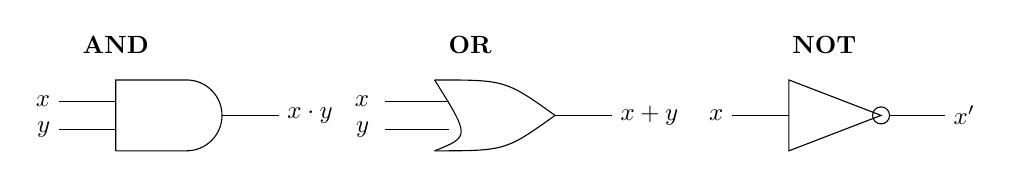
\begin{tikzpicture}[scale=0.9, transform shape]
  % --- AND Gate ---
  \node at (0, 3) {\textbf{AND}};
  \draw (0, 1.5) -- (0, 2.5) -- (1, 2.5) arc (90:-90:0.5) -- (0, 1.5);
  \draw (-0.8, 2.2) -- (0, 2.2) node[left, xshift=-0.8cm] {$x$};
  \draw (-0.8, 1.8) -- (0, 1.8) node[left, xshift=-0.8cm] {$y$};
  \draw (1.5, 2) -- (2.3, 2) node[right] {$x \cdot y$};

  % --- OR Gate ---
  \node at (5, 3) {\textbf{OR}};
  \draw (4.5, 1.5) .. controls (5,1.7) .. (4.5, 2.5);
  \draw (4.5, 2.5) .. controls (5.5,2.5) .. (6.2, 2);
  \draw (4.5, 1.5) .. controls (5.5,1.5) .. (6.2, 2);
  \draw (3.8, 2.2) -- (4.7, 2.2) node[left, xshift=-1cm] {$x$};
  \draw (3.8, 1.8) -- (4.7, 1.8) node[left, xshift=-1cm] {$y$};
  \draw (6.2, 2) -- (7, 2) node[right] {$x + y$};

  % --- NOT Gate ---
  \node at (10, 3) {\textbf{NOT}};
  \draw (9.5, 1.5) -- (9.5, 2.5) -- (10.8, 2) -- cycle;
  \draw (10.8, 2) circle (0.12);
  \draw (8.7, 2) -- (9.5, 2) node[left, xshift=-0.8cm] {$x$};
  \draw (10.92, 2) -- (11.7, 2) node[right] {$x'$};
\end{tikzpicture}
\caption{Simbol Gerbang Logika Dasar: AND, OR, dan NOT}
\label{fig:gerbang-dasar}
\end{figure}

\subsection{Kelengkapan Fungsional (Functional Completeness)}

Suatu himpunan operator Boolean dikatakan \logic{lengkap secara fungsional} (\textit{functionally complete}) jika setiap fungsi Boolean dapat diekspresikan hanya dengan menggunakan operator-operator dalam himpunan tersebut. Himpunan $\{AND, OR, NOT\}$ jelas bersifat lengkap secara fungsional karena setiap fungsi Boolean dapat ditulis dalam bentuk SOP yang hanya menggunakan ketiga operator tersebut \cite{rosen2019}.

Namun hasil yang lebih mengejutkan adalah bahwa gerbang NAND dan gerbang NOR masing-masing secara individual bersifat lengkap secara fungsional. Sifat kelengkapan fungsional NAND (dan NOR) pertama kali dibuktikan oleh Henry M. Sheffer pada tahun 1913. Artinya, seluruh rangkaian digital apa pun dapat dibangun hanya menggunakan satu jenis gerbang (NAND saja atau NOR saja). Hal ini dibuktikan dengan menunjukkan bahwa ketiga operator dasar dapat diimplementasikan hanya menggunakan NAND:

\begin{align*}
\text{NOT: } x' &= (x \cdot x)' = x \uparrow x \\
\text{AND: } x \cdot y &= ((x \cdot y)')' = (x \uparrow y) \uparrow (x \uparrow y) \\
\text{OR: } x + y &= (x' \cdot y')' = (x \uparrow x) \uparrow (y \uparrow y)
\end{align*}

Properti ini memiliki implikasi praktis yang signifikan karena dalam fabrikasi chip semikonduktor, memproduksi satu jenis gerbang secara massal lebih efisien daripada memproduksi beragam jenis gerbang. Oleh karena itu, banyak keluarga logika digital, seperti TTL (Transistor-Transistor Logic), menggunakan gerbang NAND sebagai komponen dasar \cite{allaboutcircuits_gates}.

\subsection{Dari Ekspresi Boolean ke Rangkaian Gerbang}

Proses konversi dari ekspresi aljabar Boolean ke rangkaian gerbang logika bersifat mekanistik dan langsung. Setiap operasi AND dalam ekspresi diterjemahkan menjadi gerbang AND, setiap operasi OR menjadi gerbang OR, dan setiap komplemen menjadi gerbang NOT. Interkoneksi antar gerbang mengikuti struktur ekspresi.

\begin{contoh}
\textbf{Implementasi Rangkaian untuk $F = xy + x'z$}

Ekspresi $F = xy + x'z$ memerlukan:
\begin{itemize}
    \item 1 gerbang NOT (untuk menghasilkan $x'$)
    \item 2 gerbang AND (untuk menghasilkan $xy$ dan $x'z$)
    \item 1 gerbang OR (untuk menjumlahkan kedua suku)
\end{itemize}

Total: 4 gerbang logika. Jika ekspresi ini dapat disederhanakan lebih lanjut (pada kasus ini tidak), jumlah gerbang yang diperlukan akan berkurang.
\end{contoh}

\subsection{Studi Kasus: Rangkaian Voting Mayoritas 3-Input}

\begin{contoh}
\textbf{Perancangan Rangkaian Voting Mayoritas}

Sebuah sistem voting elektronik sederhana memiliki tiga pemilih ($A$, $B$, $C$). Keputusan diambil berdasarkan suara mayoritas: output $F = 1$ jika minimal 2 dari 3 pemilih memberikan suara setuju ($= 1$).

\textbf{Langkah 1: Buat Tabel Kebenaran}

\begin{center}
\begin{tabular}{|c|c|c||c|l|}
\hline
$A$ & $B$ & $C$ & $F$ & \textbf{Keterangan} \\ \hline
0 & 0 & 0 & 0 & 0 suara setuju \\ \hline
0 & 0 & 1 & 0 & 1 suara setuju \\ \hline
0 & 1 & 0 & 0 & 1 suara setuju \\ \hline
0 & 1 & 1 & 1 & 2 suara setuju ($\geq$ mayoritas) \\ \hline
1 & 0 & 0 & 0 & 1 suara setuju \\ \hline
1 & 0 & 1 & 1 & 2 suara setuju ($\geq$ mayoritas) \\ \hline
1 & 1 & 0 & 1 & 2 suara setuju ($\geq$ mayoritas) \\ \hline
1 & 1 & 1 & 1 & 3 suara setuju ($\geq$ mayoritas) \\ \hline
\end{tabular}
\end{center}

\textbf{Langkah 2: Bentuk Kanonik SOP}
\[ F = \sum m(3, 5, 6, 7) = A'BC + AB'C + ABC' + ABC \]

\textbf{Langkah 3: Sederhanakan}
\begin{align*}
F &= A'BC + AB'C + ABC' + ABC \\
  &= A'BC + ABC + AB'C + ABC + ABC' + ABC & \text{(Idempoten)} \\
  &= BC(A' + A) + AC(B' + B) + AB(C' + C) & \text{(Distributif)} \\
  &= BC \cdot 1 + AC \cdot 1 + AB \cdot 1 & \text{(Komplemen)} \\
  &= AB + AC + BC & \text{(Identitas)}
\end{align*}

\textbf{Langkah 4: Hitung Kebutuhan Gerbang}

Ekspresi terakhir $F = AB + AC + BC$ memerlukan:
\begin{itemize}
    \item 3 gerbang AND (2-input masing-masing)
    \item 1 gerbang OR (3-input)
\end{itemize}
Total: 4 gerbang, jauh lebih sedikit dibandingkan 10+ gerbang yang dibutuhkan oleh bentuk kanonik SOP awalnya.
\end{contoh}

\subsection{Pengantar ke Bab Selanjutnya}

Meskipun metode penyederhanaan aljabar yang telah dibahas dalam bab ini sangat berguna, metode ini memiliki keterbatasan. Pertama, tidak terdapat algoritma sistematis yang menjamin bahwa solusi yang diperoleh adalah solusi optimal (paling sederhana). Kedua, untuk fungsi dengan banyak variabel dan banyak suku, proses penyederhanaan aljabar menjadi rumit dan rentan terhadap kesalahan manusia. Ketiga, kemampuan untuk ``melihat'' penyederhanaan yang tepat seringkali bergantung pada pengalaman dan intuisi perancang \cite{allaboutcircuits_boolean}.

Pada Bab~10, akan diperkenalkan \logic{Peta Karnaugh} (K-Map), sebuah metode grafis yang memberikan prosedur penyederhanaan yang lebih sistematik dan visual. Peta Karnaugh memungkinkan perancang mengidentifikasi peluang penyederhanaan melalui pengenalan pola pada peta dua dimensi, sehingga mengurangi ketergantungan pada manipulasi aljabar yang rumit. Metode ini efektif untuk fungsi hingga 4--6 variabel dan menjadi pendahulu metode algoritmik seperti algoritma Quine--McCluskey untuk fungsi dengan variabel yang lebih banyak \cite{wiki_karnaugh}.


% ============================================================
% AKTIVITAS PEMBELAJARAN
% ============================================================

\begin{aktivitas}
  \item \textbf{Postulat Huntington:} Buktikan hukum idempoten $x + x = x$ secara aljabar menggunakan postulat Huntington (ketertutupan, identitas, komplemen, distributif). Tuliskan setiap langkah beserta justifikasi postulatnya.
  \item \textbf{Tabel kebenaran:} Diberikan $F(x,y,z) = x'y + yz' + x'z$, buat tabel kebenaran lengkap (8 baris) dengan kolom antara untuk setiap subekspresi.
  \item \textbf{Penyederhanaan:} Sederhanakan $G = x'y'z + x'yz + xy'z + xyz$ menggunakan hukum-hukum aljabar Boolean. Tuliskan setiap langkah dan hukum yang digunakan.
  \item \textbf{Konversi SOP--POS:} Ubah $F(x,y,z) = \sum m(0, 2, 5, 7)$ ke bentuk kanonik POS ($\prod M$). Verifikasi dengan tabel kebenaran atau aljabar.
  \item \textbf{Hukum konsensus:} Buktikan $xy + x'z + yz = xy + x'z$ dengan hukum aljabar Boolean. Jelaskan mengapa suku $yz$ redundan.
  \item \textbf{Rangkaian gerbang:} Gambarkan rangkaian gerbang untuk $H = (A + B)(A' + C)$, sederhanakan ekspresi, lalu gambarkan rangkaian yang disederhanakan. Bandingkan jumlah gerbang sebelum dan sesudah.
  \item \textbf{Desain:} Rancang rangkaian voting mayoritas untuk 3 pemilih menggunakan hanya gerbang NAND. Tunjukkan bahwa $F = AB + AC + BC$ dapat diimplementasikan seluruhnya dengan gerbang NAND.
\end{aktivitas}

% ============================================================
% LATIHAN DAN REFLEKSI
% ============================================================

\begin{latihan}
  \item Sederhanakan $F(x, y, z) = x'y'z + x'yz + xy'$ menggunakan hukum aljabar Boolean. Tuliskan justifikasi hukum pada setiap langkah.
  \item Tuliskan bentuk minterm ($\sum m$) dan maxterm ($\prod M$) untuk $F(x, y, z) = xy + z'$. Verifikasi bahwa kedua representasi menghasilkan tabel kebenaran yang sama.
  \item Diberikan $G(A, B, C) = \sum m(1, 2, 3, 5, 7)$.
  \begin{enumerate}
    \item Tuliskan bentuk kanonik SOP lengkap.
    \item Konversikan ke bentuk kanonik POS ($\prod M$).
    \item Sederhanakan bentuk SOP menggunakan aljabar Boolean.
  \end{enumerate}
  \item Buktikan dengan aljabar Boolean: $(x + y)(x' + z)(y + z) = (x + y)(x' + z)$ (hukum konsensus versi POS).
  \item Tunjukkan bahwa gerbang NOR bersifat lengkap secara fungsional: implementasikan NOT, AND, dan OR hanya dengan gerbang NOR.
  \item Rancang fungsi Boolean untuk kontrol lampu lalu lintas sederhana: 2 sensor $S_1$, $S_2$; output lampu hijau $G$ menyala jika minimal satu sensor mendeteksi kendaraan. Tulis ekspresi Boolean, sederhanakan, dan gambarkan rangkaian gerbang.
  \item \textbf{Refleksi:} (a) Jelaskan kemiripan aljabar Boolean dengan logika proposisi dan teori himpunan; berikan contoh hukum De Morgan pada ketiga sistem. (b) Dalam pemrograman, kapan penyederhanaan ekspresi Boolean berguna? Berikan contoh kondisi \texttt{if} dalam Python yang dapat disederhanakan dengan hukum aljabar Boolean.
\end{latihan}

% ============================================================
% ASESMEN
% ============================================================

\begin{asesmen}
\textbf{Instrumen Evaluasi Kinerja (Sub-CPMK 3.1)}

\textbf{A. Pilihan Ganda}
\begin{enumerate}
  \item Hukum De Morgan untuk $(AB)'$ dalam aljabar Boolean adalah:
  \begin{enumerate}
    \item $A'B'$
    \item $A' + B'$
    \item $(A+B)'$
    \item $A+B$
  \end{enumerate}
  Jawaban: (b)

  \item Yang \emph{bukan} postulat Huntington adalah:
  \begin{enumerate}
    \item Ketertutupan
    \item Komutatif
    \item Asosiatif
    \item Distributif
  \end{enumerate}
  Jawaban: (c) --- Hukum asosiatif adalah teorema turunan.

  \item Minterm $m_5$ untuk 3 variabel $(x, y, z)$ adalah:
  \begin{enumerate}
    \item $x'y'z$
    \item $xy'z$
    \item $xyz'$
    \item $x'yz$
  \end{enumerate}
  Jawaban: (b) --- $5 = 101_2$ sehingga $x=1, y=0, z=1 \Rightarrow xy'z$.

  \item Gerbang yang lengkap secara fungsional (\textit{functionally complete}) secara individual adalah:
  \begin{enumerate}
    \item AND
    \item OR
    \item NAND
    \item XOR
  \end{enumerate}
  Jawaban: (c)

  \item Dual dari $x + (y \cdot z) = (x + y) \cdot (x + z)$ adalah:
  \begin{enumerate}
    \item $x \cdot (y + z) = (x \cdot y) + (x \cdot z)$
    \item $x' + (y' \cdot z') = (x' + y') \cdot (x' + z')$
    \item $x + (y + z) = (x + y) + z$
    \item $(x \cdot y)' = x' + y'$
  \end{enumerate}
  Jawaban: (a)
\end{enumerate}

\textbf{B. Tugas Praktik}
\begin{enumerate}
  \item Jelaskan perbedaan bentuk kanonik SOP dan POS. Kapan sebaiknya menggunakan SOP dan kapan POS?
  \item Buktikan hukum absorpsi $x + xy = x$ menggunakan postulat Huntington. Tuliskan setiap langkah beserta justifikasi postulatnya.
  \item Diberikan $F(A,B,C) = A'B'C' + A'BC + AB'C + ABC'$. Sederhanakan dengan aljabar Boolean, gambarkan rangkaian gerbang untuk ekspresi asli dan yang disederhanakan, lalu bandingkan jumlah gerbang.
\end{enumerate}

\textbf{C. Coding (opsional)}

Tulis program Python yang: (1) menerima input fungsi Boolean sebagai daftar minterm (misalnya \texttt{[1, 4, 7]} untuk 3 variabel); (2) mencetak tabel kebenaran; (3) menampilkan bentuk kanonik SOP dan POS.

\textbf{Rubrik}: Merujuk Lampiran Buku.
\end{asesmen}

% ============================================================
% CHECKLIST KOMPETENSI
% ============================================================

\begin{checklist}
  \item Saya mampu menjelaskan sejarah dan motivasi aljabar Boolean serta relasinya dengan logika proposisi dan teori himpunan.
  \item Saya memahami enam postulat Huntington dan dapat membedakannya dari teorema turunan.
  \item Saya mampu mengevaluasi fungsi Boolean untuk input tertentu dengan urutan prioritas operator yang benar.
  \item Saya menguasai hukum-hukum dasar aljabar Boolean (identitas, dominasi, idempoten, komplemen, involusi, komutatif, asosiatif, distributif, De Morgan, absorpsi, konsensus).
  \item Saya mampu menyederhanakan ekspresi Boolean secara aljabar dengan justifikasi hukum pada setiap langkah.
  \item Saya mampu membedakan literal, suku perkalian, suku penjumlahan, minterm, dan maxterm.
  \item Saya mampu mengonversi fungsi Boolean antara bentuk kanonik SOP ($\sum m$) dan POS ($\prod M$).
  \item Saya mengenal simbol dan fungsi gerbang logika dasar (AND, OR, NOT, NAND, NOR, XOR).
  \item Saya memahami kelengkapan fungsional dan dapat menjelaskan mengapa NAND atau NOR bersifat universal.
  \item Saya mampu menerjemahkan ekspresi Boolean ke rangkaian gerbang logika dan memperkirakan jumlah gerbang yang diperlukan.
\end{checklist}

% ============================================================
% RANGKUMAN
% ============================================================

\begin{rangkuman}
Bab ini mengkaji aljabar Boolean sebagai sistem aljabar yang beroperasi pada himpunan $B = \{0, 1\}$ dengan tiga operator dasar: penjumlahan Boolean (OR, $+$), perkalian Boolean (AND, $\cdot$), dan komplemen (NOT, $'$).

\textbf{Poin kunci:}
\begin{itemize}
  \item Aljabar Boolean dikembangkan oleh George Boole (1854) dan diterapkan pada analisis rangkaian digital oleh Claude Shannon (1938). Struktur ini bersifat isomorfik dengan logika proposisi dan teori himpunan, sehingga hukum pada satu kerangka dapat diterjemahkan ke kerangka lain.
  \item Postulat Huntington (1904) mendefinisikan aljabar Boolean melalui enam postulat: ketertutupan, identitas, komutatif, distributif, komplemen, dan eksistensi minimal. Hukum lain (asosiatif, idempoten, absorpsi, De Morgan, konsensus, dan sebagainya) merupakan teorema turunan.
  \item Prinsip dualitas: setiap identitas Boolean tetap valid jika $+$ dan $\cdot$ saling ditukar serta $0$ dan $1$ saling ditukar secara serentak.
  \item Penyederhanaan ekspresi dengan hukum aljabar bertujuan meminimalkan literal dan operator, sehingga mengurangi kebutuhan gerbang logika pada implementasi rangkaian.
  \item Bentuk kanonik \textit{Sum of Products} (SOP, $\sum m$) dan \textit{Product of Sums} (POS, $\prod M$) memberikan representasi standar dan saling dapat dikonversi.
  \item Gerbang logika (AND, OR, NOT, NAND, NOR, XOR) merealisasikan operator Boolean; NAND dan NOR masing-masing \textit{functionally complete}.
\end{itemize}

\textbf{Kata kunci:} aljabar Boolean, George Boole, Claude Shannon, postulat Huntington, prinsip dualitas, penyederhanaan aljabar, hukum konsensus, literal, minterm, maxterm, SOP, POS, gerbang logika, kelengkapan fungsional, NAND, NOR
\end{rangkuman}

\ifSubfilesClassLoaded{
  \renewcommand{\bibname}{Daftar Pustaka}
  \bibliographystyle{plain}
  \bibliography{../references}
}{}
\end{document}
